\documentclass[dvipsnames,table,xcdraw]{article}
\newcommand{\theHalgorithm}{\arabic{algorithm}}
\clearpage{}\usepackage{graphicx}
\usepackage{graphics}
\usepackage{amsmath}
\usepackage{amsfonts}
\usepackage{amssymb}
\usepackage{amsthm}
\usepackage{bm}
\usepackage{pgfplots}
\usepackage{adjustbox}
\usepackage{enumerate}
\usepackage{textcomp}
\usepackage{tikz}
\usepackage{tabu}
\usepackage{caption}
\usetikzlibrary{shapes, arrows, decorations.text, shadows.blur, backgrounds, positioning,fit,calc}




\usepackage{array} \usepackage{longtable} \pgfplotsset{compat=1.16}
\usepackage{microtype}
\usepackage{multirow}
\usepackage{makecell} 
\usepackage{pifont}
\newcommand{\cmark}{\ding{51}}\newcommand{\xmark}{\ding{55}}\usepackage{booktabs} \usepackage{algorithmic}
\usepackage{algorithm}
\usepackage{amsmath,amssymb,amsthm}
\usepackage{mathtools}
\newtheorem{de}{Definition}[section]
\newtheorem{theo}{Theorem}[section]
\newtheorem{prop}{Proposition}[section]
\newtheorem{lem}[theo]{Lemma}
\newenvironment{remark}[1][Remark]{\begin{trivlist}
\item[\hskip \labelsep {\bfseries #1}]}{\end{trivlist}}
\newcommand{\argmax}{\operatornamewithlimits{argmax~}}
\newcommand{\argmin}{\operatornamewithlimits{argmin~}}
\newcommand{\sinc}{\operatorname{sinc}}
\newcommand{\comb}{\operatorname{comb}}
\newcommand{\prox}[2]{\operatorname{\mathbf{prox}}_{#2}\left(#1\right)}
\newcommand{\rect}{\operatorname{rect}}
\newcommand{\erf}{\operatorname{erf}}
\newcommand{\diver}{\operatorname{div}}
\newcommand{\sgn}{\operatorname{sign}}
\newcommand{\dom}{\operatorname{dom}}
\newcommand{\trace}{\operatorname{trace}}
\newcommand{\interior}{\operatorname{int}}
\newcommand{\off}{\operatorname{off}}
\newcommand{\diag}{\operatorname{diag}}
\newcommand{\mean}{\operatorname{mean}}
\newcommand{\B}{\mathbf{B}}
\newcommand{\M}{\mathbf{M}}
\newcommand{\F}{\mathbf{F}}
\newcommand{\HH}{\mathbf{HH}}
\newcommand{\W}{\mathbf{W}}
\newcommand{\D}{\mathbf{D}}
\newcommand{\X}{\mathbf{X}}
\newcommand{\s}{\mathbf{S}}
\newcommand{\p}{\mathbf{P}}
\newcommand{\pp}{\mathbf{p}}
\newcommand{\uu}{\mathbf{u}}
\newcommand{\vv}{\mathbf{v}}
\newcommand{\xx}{\mathbf{x}}
\newcommand{\Q}{\mathbf{Q}}
\newcommand{\U}{\mathbf{U}}
\newcommand{\V}{\mathbf{V}}
\newcommand{\J}{\mathbf{J}}
\newcommand{\I}{\mathbf{I}}
\newcommand{\LL}{\mathbf{L}}
\newcommand{\PHI}{\bm{\Phi}}
\newcommand{\PSI}{\mathbf{\Psi}}
\newcommand{\LAMBDA}{\bm{\Lambda}}
\newcommand{\GAMMA}{\bm{\Gamma}}
\newcommand{\Alpha}{\bm{\alpha}}
\newcommand{\Beta}{\bm{\beta}}
\newcommand{\A}{\mathbf{A}}
\newcommand{\mb}[1]{{\boldsymbol{#1}}}
\newcommand{\vw}{\mb{w}}
\newcommand{\vb}{\mb{b}}
\newcommand{\vu}{\mb{u}}
\newcommand{\ve}{\mb{e}}
\newcommand{\vy}{\mb{y}}
\usepackage{bbm}
\newcommand{\balpha}{\bm{\alpha}}
\newcommand{\bbeta}{\bm{\beta}}
\newcommand{\btau}{\bm{\tau}}
\newcommand{\brho}{\bm{\rho}}

\newcommand{\bgamma}{\bm{\gamma}}
\newcommand{\bdelta}{\bm{\delta}}
\newcommand{\bDelta}{\bm{\Delta}}
\newcommand{\bs}{\bm{s}}

\newenvironment{disarray}{\everymath{\displaystyle\everymath{}}\array}{\endarray}
\usepackage{pgfpages}



\newcommand{\norm}[1]{\lVert #1 \rVert}
\usepackage{relsize}
\usepackage{lmodern}


\setlength{\intextsep}{0em}
\setlength{\parskip}{0.3em}
\setlength{\dblfloatsep}{-3em}
\setlength{\dbltextfloatsep}{-3em}

\setlength{\abovecaptionskip}{0.7em}
\setlength{\belowcaptionskip}{-1em}
\usepackage[nodisplayskipstretch]{setspace}
\setstretch{0.99}

\AtBeginDocument{\setlength\abovedisplayskip{4pt}
  \setlength\belowdisplayskip{4pt}
  }



\usepackage{listings}

\definecolor{codegreen}{rgb}{0,0.6,0}
\definecolor{codegray}{rgb}{0.5,0.5,0.5}
\definecolor{codepurple}{rgb}{0.58,0,0.82}
\definecolor{backcolour}{rgb}{0.95,0.95,0.92}

\lstdefinestyle{mystyle}{
    backgroundcolor=\color{backcolour},   
    commentstyle=\color{codegreen},
    keywordstyle=\color{magenta},
    numberstyle=\tiny\color{codegray},
    stringstyle=\color{codepurple},
    basicstyle=\ttfamily\footnotesize,
    breakatwhitespace=false,         
    breaklines=true,                 
    captionpos=b,                    
    keepspaces=true,                 
    numbers=left,                    
    numbersep=5pt,                  
    showspaces=false,                
    showstringspaces=false,
    showtabs=false,                  
    tabsize=2
}

\lstset{style=mystyle}
\definecolor{darkbluetemp}{rgb}{0,0.08,0.45}
\usepackage[colorlinks=true, allcolors=darkbluetemp]{hyperref}
\clearpage{}
\usepackage[accepted]{icml2021arxiv}

\icmltitlerunning{HardCoRe-NAS}


\usepackage{cleveref}[2012/02/15]\crefformat{footnote}{#2\footnotemark[#1]#3}

\begin{document}
\twocolumn[
\icmltitle{HardCoRe-NAS: Hard Constrained diffeRentiable\\Neural Architecture Search}
\icmlsetsymbol{equal}{*}
\begin{icmlauthorlist}
\icmlauthor{Niv Nayman}{equal,to}
\icmlauthor{Yonathan Aflalo}{equal,to}
\icmlauthor{Asaf Noy}{to}
\icmlauthor{Lihi Zelnik-Manor}{to}
\end{icmlauthorlist}
\icmlaffiliation{to}{Alibaba Group, Tel Aviv, Israel}
\icmlcorrespondingauthor{Niv Nayman}{niv.nayman@alibaba-inc.com}
\icmlcorrespondingauthor{Yonathan Aflalo}{johnaflalo@gmail.com}
\icmlkeywords{Machine Learning, ICML}
\vskip 0.16in
]
\printAffiliationsAndNotice{\icmlEqualContribution} \begin{abstract}
Realistic use of neural networks often requires adhering to multiple constraints on latency, energy and memory among others.
A popular approach to find fitting networks is through constrained Neural Architecture Search (NAS), however, previous methods enforce the constraint only softly. 
Therefore,  the resulting networks do not exactly adhere to the resource constraint and their accuracy is harmed.
In this work we resolve this by introducing \textit{Hard Constrained diffeRentiable NAS (HardCoRe-NAS)}, that is based on an accurate formulation of the expected resource requirement and a scalable search method that satisfies the hard constraint throughout the search.
Our experiments show that HardCoRe-NAS generates state-of-the-art architectures, surpassing other NAS methods, while strictly satisfying the hard resource constraints without any tuning required.
\end{abstract}



%
 \begin{figure}[t]
\begin{adjustbox}{width=0.5\textwidth}
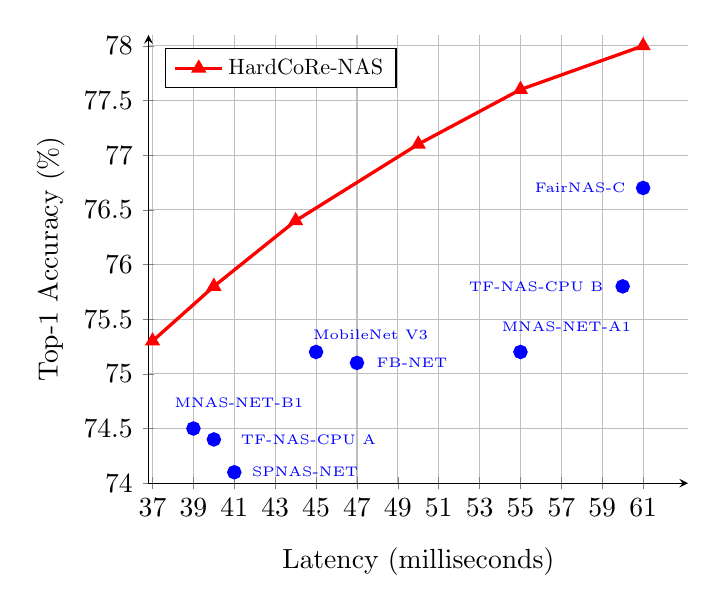
\begin{tikzpicture}
\begin{axis}[
axis x line=left,
            axis y line=left,
            xmajorgrids=true,
            ymajorgrids=true,
            grid=both,
            xlabel style={below=1ex},
            enlarge x limits,
            ymin = 74.0,
            ymax = 78.1,
xmin = 39.0,
            xmax = 61.0,
xtick = {37,39,...,61},
ytick = {74.0,74.5,...,78.1},
            ylabel = Top-1 Accuracy (\%),
            xlabel = Latency  (milliseconds),
            legend pos=north west,
            legend style={nodes={scale=0.8, transform shape}}
]




\addplot[color=red, mark=triangle*,very thick]coordinates {(37, 75.3)(40,75.8)(44, 76.4)(50, 77.1)(55, 77.6)(61,78.0)};\addlegendentry{HardCoRe-NAS}









\addplot[only marks,color=blue,mark=*,very thick]coordinates {(45, 75.2)} node (MobileNet_V3){};
\node[color=blue, above right = -0.1cm and -0.3cm of MobileNet_V3, font=\tiny] {MobileNet V3};

\addplot[only marks,color=blue,mark=*,very thick]coordinates {(40, 74.4)} node (tfnasa){};
\node[color=blue, right of=tfnasa, font=\tiny, node distance = 1.2cm] {TF-NAS-CPU A};

\addplot[only marks,color=blue,mark=*,very thick]coordinates {(60, 75.8)} node (tfnasb){};
\node[color=blue, left of=tfnasb, font=\tiny, node distance = 1.1cm] {TF-NAS-CPU B};



\addplot[only marks,color=blue,mark=*,very thick]coordinates {(55, 75.2)} node (mnasa1){};
\node[color=blue, above right = 0.0cm and -0.5cm of mnasa1, font=\tiny, node distance = 0.01cm] {MNAS-NET-A1};

\addplot[only marks,color=blue,mark=*,very thick]coordinates {(39, 74.5)} node (mnasb1){};
\node[color=blue, above right = 0.0cm and -0.5cm of mnasb1, font=\tiny, node distance = 0.01cm] {MNAS-NET-B1};

\addplot[only marks,color=blue,mark=*,very thick]coordinates {(41, 74.1)} node (spnas){};
\node[color=blue, right of=spnas, font=\tiny, node distance = 0.9cm] {SPNAS-NET};





\addplot[only marks,color=blue,mark=*,very thick]coordinates {(47, 75.1)} node (fbnet){};
\node[color=blue, right of=fbnet, font=\tiny, node distance = 0.7cm] {FB-NET};


\addplot[only marks,color=blue,mark=*,very thick]coordinates {(61, 76.7)} node (FairNASC){};
\node[color=blue, left of=FairNASC, font=\tiny, node distance = 0.8cm] {FairNAS-C};




\end{axis}
\end{tikzpicture}
\end{adjustbox}
\vspace*{-7mm}
\caption{Top-1 accuracy on Imagenet vs Latency measured on Intel Xeon CPU for a batch size of 1. HardCoreNAS can generate a network for any given latency, with accuracy according to the red curve, which is higher than all previous methods.}
\label{fig:acc_nas}
\end{figure}




 \section{Introduction}
With the rise in popularity of Convolutional Neural Networks (CNN), the need for neural networks with fast inference speed and high accuracy, has been growing continuously. At first, manually designed architectures, such as VGG~\cite{VGG} or ResNet~\cite{ResNet}, targeted powerful GPUs as those were the common computing platform for deep CNNs. Many variants of those architectures were the golden standard until the need for deployment on edge devices and standard CPUs emerged. These are more limited computing platforms, requiring lighter architectures that for practical scenarios have to comply with hard constraints on the real time latency or power consumption. This has spawned a line of research aimed at finding architectures with both high performance and bounded resource demand. 

The main approaches to solve this evolved from Neural Architecture Search (NAS)~\cite{zoph2016neural, liu2018darts, cai2018proxylessnas}, while adding a constraint on the target latency over various platforms, e.g., TPU, CPU, Edge-GPU, FPGA, etc. 
The constrained-NAS methods can be grouped into two categories: (i) Reward based methods such as Reinforcement-Learning (RL) or Evolutionary Algorithm (EA) \cite{OFA,tan2019mnasnet, effnet, mobilenetv3}, where the search is performed by sampling networks and predicting their final accuracy and resource demands by evaluation over some validation set. The predictors are expensive to acquire and oftentimes inaccurate. (ii) Resource-aware gradient based methods \cite{TF-NAS,fbnet} formulate a differentiable loss function consisting of a trade-off between an accuracy term and a proxy soft penalty term. Therefore, the architecture can be directly optimized using stochastic gradient descent (SGD)~\cite{SGD}, however, it is hard to tune the trade-off between accuracy and resources, which deteriorates the network accuracy and fails to fully meet the resource requirements. 
The hard constraints over the resources are further violated due to a final discretization step projecting the architecture over the differentiable search space into the discrete space of architectures.
 
In this paper, we propose a search algorithm that produces architectures with high accuracy (Figure~\ref{fig:acc_nas}) that strictly satisfy any given hard latency constraint (Figure~\ref{fig:latency}). The search algorithm is fast and scalable to a large number of platforms. The proposed algorithm is based on several key ideas, starting from formulating the NAS problem more accurately, accounting for hard constraints over resources, and solving every aspect of it rigorously. For clarity we focus in this paper on latency constraints, however, our approach can be generalized to other types of resources.

 At the heart of our approach lies a suggested differentiable search space that induces a one-shot model~\cite{bender2018understanding, fairnas, SPOS, OFA} that is easy to train via a simple, yet effective, technique for sampling multiple sub-networks from the one-shot model, such that each one is properly pretrained. 
 We further suggest an accurate formula for the expected latency of every architecture residing in that space. Then, we search the space for sub-networks by solving a hard constrained optimization problem while keeping the one-shot model pretrained weights frozen. We show that the constrained optimization can be solved via the block coordinate stochastic Frank-Wolfe (BC-SFW) algorithm~\cite{SFW,BCFW}. Our algorithm converges faster than SGD, while tightly satisfying the hard latency constraint continuously throughout the search, including during the final discretization step.
 
 The approach we propose has several advantages. First, the outcome networks provide high accuracy and closely comply to the latency constraint. 
 In addition, our solution is scalable to multiple target devices and latency demands. This scalability is due to the efficient pretraining of the one-shot model as well as the fast search method that involves a relatively small number of parameters, governing only the structure of the architecture. 
 We hope that our formulation of NAS as a constrained optimization problem, equipped with an efficient algorithm that solves it, could give rise to followup work incorporating a variety of resource and structural constraints over the search space.  \section{Related Work}
\textbf{Efficient Neural Networks} are designed to meet the rising demand of deep learning models for numerous tasks per hardware constraints. Manually-crafted architectures such as MobileNets~\cite{howard2017mobilenets,sandler2018mobilenetv2} and ShuffleNet~\cite{zhang2018shufflenet} were designed for mobile devices, while TResNet~\cite{ridnik2020tresnet} and ResNesT~\cite{zhang2020resnest} are tailor-made for GPUs. Techniques for improving efficiency include pruning of redundant channels~\cite{dong2019network,aflalo2020knapsack} and layers~\cite{han2015learning}, model compression~\cite{han2015deep, he2018amc} and weight quantization methods~\cite{hubara2016binarized,umuroglu2017finn}. Dynamic neural networks adjust models based on their inputs to accelerate the inference, via gating modules~\cite{wang2018skipnet}, graph branching~\cite{huang2017multi} or dynamic channel selection~\cite{lin2017runtime}. These techniques are applied on  predefined architectures, hence cannot utilize or satisfy specific hardware constraints. 

\textbf{Neural Architecture Search} methods automate models' design per provided constraints. Early methods like NASNet~\cite{zoph2016neural} and AmoebaNet~\cite{real2019regularized} focused solely on accuracy, producing SotA classification models~\cite{huang2019gpipe} at the cost of GPU-years per search, with relatively large inference times. DARTS~\cite{liu2018darts} introduced a differential space for efficient search and reduced the training duration to days, followed by XNAS~\cite{nayman2019xnas} and ASAP~\cite{noy2020asap} that applied pruning-during-search techniques to further reduce it to hours. 
Hardware-aware methods such as ProxylessNAS~\cite{cai2018proxylessnas}, Mnasnet~\cite{tan2019mnasnet}, FBNet~\cite{fbnet} and TFNAS~\cite{TF-NAS} 
produce architectures that satisfy the required constraints by applying simple heuristics such as soft penalties on the loss function.
OFA~\cite{OFA} proposed a scalable approach across multiple devices by training an one-shot model~\cite{brock2017smash,bender2018understanding} for 1200 GPU hours. This provides a strong pretrained super-network being highly predictive for the accuracy of extracted sub-networks~\cite{SPOS,fairnas,yu2020train}. This work relies on such one-shot model acquired within only 400 GPU hours in a much simpler manner and satisfies hard constraints tightly with less heuristics.



\textbf{Frank-Wolfe (FW) algorithm}~\cite{frank_wolfe} 
is commonly used by machine learning applications~\cite{sun2019survey} thanks to its projection-free property~\cite{combettes2020projection,hazan2020faster} and ability to handle structured constraints~\cite{jaggi2013revisiting}. Modern adaptations aimed at deep neural networks (DNNs) optimization include more efficient variants~\cite{zhang2020quantized,combettes2020projection}, task-specific variants~\cite{chen2020frank,tsiligkaridis2020frank}, as well as improved convergence guarantees~\cite{lacoste2015global,d2020global}. Two prominent variants are the stochastic FW~\cite{hazan2016variance} and Block-coordinate FW~\cite{lacoste2013block}.
While FW excels as an optimizer for DNNs~\cite{berrada2018deep,pokutta2020deep}, this work is the first to utilize it for NAS.





% \vspace{-1.5mm}
\section{Method} \label{sec:method}
In the scope of this paper, we focus on latency-constrained NAS, searching for an architecture with the highest validation accuracy under a predefined latency constraint, denoted by . Our architecture search space  is parametrized by , governing the architecture structure in a fully differentiable manner, and , the convolution weights.
A latency-constrained NAS can be expressed as the following constrained bilevel optimization problem:

where  and  are the train and validation sets' distributions respectively,  is some probability measure over the search space parameterized by ,  is the cross entropy loss as a differentiable proxy for the negative accuracy and  is the estimated latency of the model.

To solve problem~\eqref{eqn:NAS_bilevel}, we construct a fully differentiable search space parameterized by  (Section~\ref{sec:search_space}), that enables the formulation of a differentiable closed form formula expressing the estimated latency  (Section~\ref{sec:latency_formula}) and efficient acquisition of  (Section~\ref{sec:inner_problem}). Finally, we introduce rigorous constrained optimization techniques for solving the outer level problem (Section~\ref{sec:outer_problem}).

\subsection{Search Space}
\label{sec:search_space}
Aiming at the most accurate latency, a flexible search space is composed of a micro search space that controls the internal structures of each block , together with a macro search space that specifies the way those are connected to one another in every stage .

\subsubsection{Micro-Search}\label{sec:micro_search}
Every block is an \textit{elastic} version of the MBInvRes block, introduced in~\cite{mobilenetv2}, with expansion ratio  of the point-wise convolution, kernel size  of the depth-wise separable convolution (DWS), and Squeeze-and-Excitation (SE) layer~\cite{SE} .
The blocks are configurable, as illustrated at the bottom of Figure~\ref{fig:super_net}, using a parametrization , defined for every block  of stage :

\begin{figure}[t]
  \centering
  \includegraphics[width=0.45\textwidth]{images/search_space.pdf}
\caption{A search space view via the one-shot model}
\label{fig:super_net}
\end{figure}
Each triplet  induces a block configuration  that resides within a micro-search space , parameterized by  , where  denotes the Cartesian product. Hence, for each block  of stage  we have:

An input feature map  to block  of stage  is processed as follows:

where  is the operation performed by the elastic MBInvRes block configured according to .

Having several configurations  share the same values of  or  or  induces weight sharing between the common operations of the associated architectures. This weight sharing is beneficial for solving the inner problem~\eqref{eqn:NAS_bilevel} effectively, as will be discussed in Section~\ref{sec:inner_problem}.


\subsubsection{Macro-Search}\label{sec:macro_search}
Inspired by~\cite{TF-NAS, OFA}, the output of each block of every stage is also directed to the end of the stage as illustrated in the middle of Figure~\ref{fig:super_net}. Thus, the depth of each stage  is controlled by the parameters , such that:

The depth is , since:


\subsubsection{The Composed Search Space}\label{sec:composed_search_space}
The overall search space is composed of both the micro and macro search spaces parameterized by  and , respectively, such that:


A continuous probability distribution is induced over the space, by relaxing  and  to be continuous rather than discrete.
A sample sub-network is drawn  using the Gumbel-Softmax Trick~\cite{GumbelSM} such that , as specified in~\eqref{eqn:gumbel_alpha} and~\eqref{eqn:gumbel_beta}.
In summary, one can view the parametrization  as a composition of probabilities in  or as degenerated one-hot vectors in .

Effectively we include at least a couple of blocks in each stage by setting , hence, the overall size of the search space is:



\subsection{Formulating the Latency Constraint}
\label{sec:latency_formula}
Aiming at tightly satisfying latency constraints, we propose an accurate formula for the expected latency of a sub-network. The expected latency of a block  can be computed by summing over the latency  of every possible configuration :

Thus the expected latency of a stage of depth  is 

Taking the expectation over all possible depths yields  

and summing over all the stages results in the following formula for the overall latency:

The the summation originated in \eqref{eqn:latency_correction} differentiates our latency formulation~\eqref{eqn:latency_formula} from that of~\cite{TF-NAS}. 


Figure~\ref{fig:latency} provides empirical validation of~\eqref{eqn:latency_formula}, showing that in practice the actual and estimated latency are very close on both GPU and CPU. More details on the experiments are provided in Section~\ref{sec:validate_latency}.

\begin{figure}[t]
\centering
\begin{adjustbox}{width=0.47\textwidth}
\begin{tikzpicture}
\begin{axis}[
axis x line=left,
            axis y line=left,
            xmajorgrids=true,
            ymajorgrids=true,
            grid=both,
            xlabel style={below=1ex},
            enlarge x limits,
            ymin = 24.0,
            ymax = 66,
            xmin = 24.0,
            xmax = 66,
xtick = {25,30,...,65},
            ytick = {25,30,...,65},
            ylabel = Measured Latency (milliseconds),
            xlabel = Latency Formula (milliseconds),
            legend pos=north west,
            legend style={nodes={scale=0.8, transform shape}}
]


\addplot[only marks, color=red, mark=triangle*,very thick]coordinates {(25, 27)(30, 32)(35, 36)(40, 42)}	
;\addlegendentry{GPU}

\addplot[only marks, color=blue, mark=triangle*,very thick]coordinates {
(35, 35.36)
(40, 42.63)
(45, 47.45)
(50, 54.51)
(55, 56.98)
(60, 61.93)
(65, 64.03)
};\addlegendentry{CPU}

\addplot[style=dashed, color=ForestGreen, very thick]coordinates {(24,24)(66, 66)};
\addplot[color=ForestGreen,very thick]coordinates {(55,35)} node (kendal_tau_ours_100){

};
\end{axis}
\end{tikzpicture}
\end{adjustbox}
\vspace*{-3mm}
\caption{Experimental results showing that the latency calculated with formula~\eqref{eqn:latency_formula} is very close to the latency measured in practice, on both CPU and GPU.}
\label{fig:latency}
\end{figure}
 


\textbf{Remark:} By replacing the latency measurements  with other resources, e.g., memory, FLOPS, MACS, etc., one can use formula~\eqref{eqn:latency_formula} to add multiple hard constraints to the outer problem of~\eqref{eqn:NAS_bilevel}.

\subsection{Solution to the Inner Problem }
\label{sec:inner_problem}
Previous work proposed approximated solutions to the following unconstrained problem:

typically by alternating or simultaneous updates of  and  \cite{liu2018darts, SNAS, cai2018proxylessnas, fbnet, TF-NAS}.
This approach has several limitations.
First, obtaining a designated  with respect to every update of  involves a heavy training of a neural network until convergence. Instead a very rough approximation is obtained by just a few update steps for .
In turn, this approximation creates a bias towards strengthening networks with few parameters since those learn faster, hence, get sampled even more frequently, further increasing the chance to learn in a positive feedback manner. Eventually, often overly simple architectures are generated, e.g., consisting of many skip-connections~\cite{P-DARTS, DARTS+}. Several remedies have been proposed, e.g., temperature annealing, adding uniform sampling, modified gradients and updating only  for a while before the joint optimization begins~\cite{noy2020asap, fbnet, TF-NAS, nayman2019xnas}. While those mitigate the bias problem, they do not solve it.

We avoid such approximation whatsoever. Instead we obtain  of the inner problem of~\eqref{eqn:NAS_bilevel} only once, with respect to a uniformly distributed architecture, sampling  from .

This is done by sampling multiple distinctive paths (sub-networks of the one-shot model) for every image in the batch in an efficient way (just a few lines of code provided in the supplementary materials), using the Gumbel-Softmax Trick. 
For every feature map  that goes through block  of stage , distinctive uniform random variables  are sampled, governing the path undertaken by this feature map:





Based on the observation that the accuracy of a sub-network with  should be predictive for its accuracy when optimized as a stand-alone model from scratch, we aim at an accurate prediction.
Our simple approach implies that, with high probability, the number of paths sampled at each update step is as high as the number of images in the batch. This is two orders of magnitude larger than previous methods that sample a single path per update step \cite{SPOS, OFA}, while avoiding the need to keep track of all the sampled paths \cite{fairnas}. Using multiple paths reduces the variance of the gradients with respect to the paths sampled by an order of magnitude\footnote{A typical batch consists of hundreds of i.i.d paths, thus a variance reduction of the square root of that is in place.}. Furthermore, leveraging the weight sharing implied by the structure of the elastic MBInvRes block (Section~\ref{sec:micro_search}), the number of gradients observed by each operation is increased by a factor of at least . This further reduces the variance by half. 

\begin{figure}[t]
\begin{adjustbox}{width=0.47\textwidth}
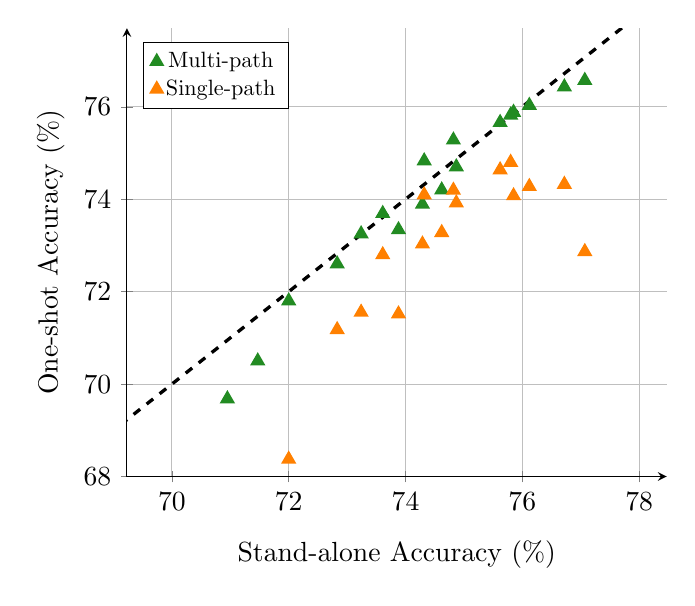
\begin{tikzpicture}
\begin{axis}[
axis x line=left,
            axis y line=left,
            xmajorgrids=true,
            ymajorgrids=true,
            grid=both,
            xlabel style={below=1ex},
            enlarge x limits,
ymin = 68.0,
            ymax = 77.7,
xmin = 70.0,
            xmax = 77.7,
xtick = {68,67,...,78},
            ytick = {68,67,...,78},
            ylabel = One-shot Accuracy (\%),
            xlabel = Stand-alone Accuracy (\%),
            legend pos=north west,
            legend style={nodes={scale=0.8, transform shape}}
]


\addplot[only marks, color=ForestGreen, mark=triangle*,very thick]coordinates {(70.95,69.68)(71.47, 70.5)(72, 71.8)(72.83, 72.60)(73.88, 73.34)(74.29, 73.89)
(73.24,73.25)(73.61,73.69)(74.32, 74.83)(74.82, 75.28)(75.80, 75.82)(76.12,76.03)
(74.62, 74.2)(74.87,74.7 )(75.62,75.66)(75.85,75.88)(76.72,76.43)(77.07,76.57)};\addlegendentry{Multi-path} 








\addplot[only marks, color=orange, mark=triangle*,very thick]coordinates {(70.95,61.036)(71.47,65.73)(72,68.374)(72.83,71.178)(73.88,71.518)(74.29,73.03)
(73.24,71.554)(73.61,72.798)(74.32,74.094)(74.82,74.194)(75.80,74.798)(76.12,74.274)
(74.62,73.278)(74.87,73.92)(75.62,74.636)(75.85,74.074)(76.72,74.322)(77.07,72.866)};\addlegendentry{Single-path} 






\addplot[style=dashed, color=black, very thick]coordinates {(66, 66)(78, 78)};

\addplot[color=ForestGreen,very thick]coordinates {(71,74)} node (kendal_tau_ours_100){\makecell{\\ }};





\addplot[color=orange,very thick]coordinates {(76, 70)} node (kendal_tau_other3){\makecell{\\ }};






\end{axis}
\end{tikzpicture}
\end{adjustbox}
\vspace*{-3mm}
\caption{Top-1 accuracy on Imagenet of networks trained from scratch v.s. corresponding sub-networks extracted from our one-shot model.  and  represent the Kendall-Tau and Spearman correlation coefficients, respectively.}
\label{fig:acc_kendal_tau}
\end{figure} Figure~\ref{fig:acc_kendal_tau} shows that we obtain a one-shot model  with high correlation between the ranking of sub-networks directly extracted from it and the corresponding stand-alone counterpart trained from scratch. See more details in Section~\ref{sec:evaluate_inner}. This implies that  captures well the quality of sub-structures in the search space.
\subsection{Solving the Outer Problem}
\label{sec:outer_problem}
Having defined the formula for the latency LAT and obtained a solution for , we can now continue to solve the outer problem~\eqref{eqn:NAS_bilevel}. 

\subsubsection{Searching Under Latency Constraints}
Most differentiable resource-aware NAS methods account for the resources through shaping the loss function with soft penalties~\cite{fbnet, TF-NAS}. This approach solely does not meet the constraints tightly.
Experiments illustrating this are described in Section~\ref{subsec:toy_example}.

Our approach directly solves the constrained outer problem~\eqref{eqn:NAS_bilevel}, hence, it enables the strict satisfaction of resource constraints by further restricting the search space, i.e.,
.

As commonly done for gradient based approaches, e.g.,~\cite{liu2018darts}, we relax the discrete search space  to be continuous by searching for .
As long as  is convex, it could be leveraged for applying the stochastic Frank-Wolfe (SFW) algorithm~\cite{SFW} to directly solve the constrained outer problem:

following the update step:

where  and  are the sampled data and the learning rate at step , respectively.
For  of linear constraints, the linear program~\eqref{eqn:lp} can be solved efficiently, using the Simplex algorithm~\cite{simplex}.

A convex  together with  satisfy  anytime, as long as .
We provide a method for satisfying the latter in the supplementary materials.

The benefits of such optimization are demonstrated in Figure~\ref{fig:fw_vs_gd} through a toy problem, described in Section~\ref{subsec:toy_example}. While GD is sensitive to the trade-off involved with a soft penalty, FW converges faster to the optimum with zero penalty. 

\begin{figure}[htb]
    \centering
    \includegraphics[width=0.47\textwidth]{images/gd_diff_lambda.pdf}
    \caption{Objective loss and soft penalty for FW and GD for different values of the penalty coefficient . Solid and dashed curves represent the objective loss (left y-axis) and soft penalty (right y-axis), respectively. FW converges to the optimum much faster than GD.}
    \label{fig:fw_vs_gd}
\end{figure}


All this requires  to be convex. 
While  is obviously convex, formed by linear constraints, the latency constraint  is not necessarily so. The latency formula \eqref{eqn:latency_formula} can be expressed as a quadratic constraint by constructing a matrix  from , such that,

Since  is constructed from measured latency, it is not guaranteed to be positive semi-definite, hence, the induced quadratic constraint could make  non-convex.

To overcome this, we introduce the Block Coordinate Stochastic Frank-Wolfe (BCSFW) Algorithm~\ref{alg:BCSFW}, that combines Stochastic Frank-Wolfe with Block Coordinate Frank-Wolfe~\cite{BCFW}. This is done by forming separated convex feasible sets at each step, induced by linear constraints only:

 This implies that  for all .
Moving inside the feasible domain at anytime avoids irrelevant infeasible structures from being promoted and hiding feasible structures.
\vspace{1em}
\begin{algorithm}[htb]
   \caption{Block Coordinate SFW (BCSFW)}
   \label{alg:BCSFW}
\begin{algorithmic}
\INPUT 
\FOR{}
\STATE Pick  or  at random
\STATE Sample an i.i.d validation batch 
\STATE 
\STATE Update  with 
\ENDFOR
\end{algorithmic}
\end{algorithm}
 








\subsubsection{Projection Back to the Discrete Space}\label{sec:projection}
As differentiable NAS methods are inherently associated with a continuous search space, a final discretizaiton step  is required for extracting a single architecture. 
Most methods use the \textit{argmax} operator:

for all , where  is the solution to the outer problem of~\eqref{eqn:NAS_bilevel}.


For resource-aware NAS methods, applying such projection results in possible violation of the resource constraints, due to the shift from the converged solution in the continuous space. Experiments showing that latency constraints are violated due to~\eqref{eqn:argmax} are provided in Section~\ref{sec:projection_effect}.

While several methods mitigate this violation by promoting sparse probabilities during the search, e.g.,~\cite{noy2020asap, nayman2019xnas}, 
our approach completely eliminates it by introducing an alternative projection step, described next.

Viewing the solution of the outer problem  as the credit assigned to each configuration,
we introduce a projection step that maximizes the overall credit while strictly satisfying the latency constraints. It is based on solving the following two linear programs:

Note, that when there is no latency constraint, e.g., , \eqref{eqn:projection_step} coincides with~\eqref{eqn:argmax}.

We next provide a theorem that guarantees that the projection~\eqref{eqn:projection_step} yields a sparse solution, representing a valid sub-network of the one-shot model. Specifically, a single probability vector from those composing  and  contains up to two non-zero entries each, as all the rest are one-hot vectors. 
\begin{theo}
\label{thm:one_hot_sol}
The solution  of \eqref{eqn:projection_step} admits:

where  and , ,   are single block and stage respectively, satisfying:

\end{theo}
Refer to the supplementary materials for the proof.

\textbf{Remark:} A negligible deviation is associated with taking the argmax~\eqref{eqn:argmax} over the only two couples referred to in~\eqref{eqn:dense_remiders}. Experiments supporting this are described in Section~\ref{sec:projection_effect}. Furthermore, this can be entirely eliminated by solving an equivalent Multiple-Choice Knapsack Problem (MCKP) as described in the supplementary material.










































































 \section{Experimental Results}\label{sec:experiments}

\subsection{Search for State-of-the-Art Architectures}
\subsubsection{Dataset and Setting} \label{sec:exp_setting}
For all of our experiments, we train our networks using SGD with a learning rate of  with cosine annealing, Nesterov momentum of , weight decay of , applying label smoothing \cite{label_smoothing} of 0.1, mixup \cite{mixup} of 0.2, Autoaugment \cite{autoaugment}, mixed precision and EMA-smoothing.

We obtain the solution of the inner problem  as specified in sections \ref{sec:inner_problem} and \ref{sec:evaluate_inner} over 80\% of a random 80-20 split of the ImageNet train set. We utilize the remaining 20\% as a validation set and search for architectures with latencies of  and  milliseconds running with a batch size of 1 and 64 on an Intel Xeon CPU and and NVIDIA P100 GPU, respectively. The search is performed according to section \ref{sec:outer_problem} for only 2 epochs of the validation set, lasting for 8 GPU hours\cref{fn:batch_16}. 
\vspace{-0.2em}
\subsubsection{Comparisons with other methods}\label{sec:exp_comparison}
\vspace{-0.2em}
We compare our generated architectures to other state-of-the-art NAS methods in Table~\ref{tab:exp} and Figure~\ref{fig:acc_nas}. 
For each model in the table, we use the official PyTorch implementation \cite{pytorch} and measure its latency running on a single thread with the exact same conditions as for our networks. We excluded further optimizations, such as Intel MKL-DNN~\cite{mkl_dnn}, therefore, the latency we report may differ from the one originally reported. 
For the purpose of comparing the generated architectures alone, excluding the contribution of evolved pretraining techniques, all the models (but OFA\cref{fn:ofa}) are trained from a random initialization with the same settings, specified in section~\ref{sec:exp_setting}. 
It can be seen that networks generated by our method meet the latency target closely, while at the same time surpassing all the others methods on the top-1 accuracy over ImageNet with a reduced scalable search time. 







\begin{table}[t]
\small
    \centering
    \begin{tabular}{c|l|c|c|c|}
    & Model & \makecell[c]{Latency \\ (ms)} & \makecell[c]{Top-1 \\ (\%)} & \makecell[c]{Total  Cost\
    \label{eqn:toy_ex}
    \min_x \|x\|^2  \quad \text{s.t. }\ 
       \Sigma_{i=1}^d x_i = 1 \quad ; \quad x\in\mathbb{R}^d
\label{eqn:toy_fw_step}
x_{t+1} &= (1-\gamma_t)\cdot x_t + \gamma_t\cdot\xi_t\\
\xi_t &=\argmin_x \|x\|^2 \text{ s.t. } \Sigma_{i=1}^d x_i = 1
\label{eqn:er_sum}
    y^s_{b, er} = \sum_{er\in\mathcal{A}_{er}} \alpha^s_{b, er}\cdot PWC^s_{b,er}(x^s_b)
\label{eqn:er_sum_mask}
    y^s_{b, er} = \sum_{er\in\mathcal{A}_{er}} \alpha^s_{b, er}\cdot PWC^s_{b,\bar{er}}(x^s_b)\odot \mathbbm{1}_{C\leq er\times C_{in}}

    \label{eqn:FW}
    \min_{\mathbf{x} \in \mathcal{D}}f(\mathbf{x}).

    \label{eqn:FW2}
    \min_{\mathbf{x_k+\bDelta} \in \mathcal{D}}f(\mathbf{x_k+\bDelta}).

    \label{eqn:FW3}
    \min_{\mathbf{x_k+\bDelta} \in \mathcal{D}}\bDelta^T\nabla f(\mathbf{x_k})

    \label{eqn:FW4}
    \min_{\mathbf{\mathbf{x_k}+\gamma (\bs-\mathbf{x_k})} \in \mathcal{D}}\gamma (s-\mathbf{x_k})^T\nabla f(\mathbf{x_k}).

    \label{eqn:FW_step}
    \min_{\mathbf{s} \in \mathcal{D}}s^T\nabla f(\mathbf{x_k}).

\label{eqn:FW_update}
\mathbf{x}_{k+1}\leftarrow \mathbf{x}_k+\gamma(\mathbf{s}_k-\mathbf{x}_k).
\label{eqn:trivial_init}
    \tilde{\alpha}^s_{b,c}=\mathbbm{1}\{c=1\} \, ; \, \tilde{\beta}^s_b=\mathbbm{1}\{b=2\}
\label{eqn:qp_init}
  &\min_{\vu\in\mathcal{S}^{\tilde{\vu}}} \sum_{s=1}^s \sum_{b=1}^{d-1}\sum_{c=1}^{|\mathcal{C}|-1} (\alpha^s_{b,c+1}-\alpha^s_{b,c})^2 
  \\
  &\min_{\bbeta\in\mathcal{S}^{\tilde{\bbeta}}} \sum_{s=1}^s \sum_{b=1}^{d-1}(\beta^s_{b+1}-\beta^s_{b})^2
  \notag

\label{eqn:qp_init_vs_lightest}
\frac{100}{|\mathcal{T}|} \sum_{T\in\mathcal{T}} \frac{Acc^T_{\text{balance init}} - Acc^T_{\text{lighest init}}}{Acc^T_{\text{lighest init}}}

\label{eqn:MCKP}
\notag
\max_{vu} &\sum_{i=1}^k \sum_{j\in N_i}  p_{ij} \vu_{ij} \\
\text{subject to}
&\sum_{i=1}^k\sum_{j\in N_i} t_{ij} \vu_{ij} \leq T \\
\notag
&\sum_{j \in N_i}\vu_{ij} = 1 \qquad \forall i \in \{1,\dots,k\} \\
\notag
&\vu_{ij} \geq 0  \qquad \forall i \in \{1,\dots,k\}, j \in N_i
||\vu_i^*||^0=\sum_{j\in N_i} |\vu_{ij}^*|^0=\sum_{j\in N_i}\mathbbm{1}_{\vu_{ij}^*>0}=1\label{eqn:q}
 q&=\frac{t_{i_2 j_2}-t_{i_1 j_1}}{t_{i_2 j_3}-t_{i_2 j_4}} 
 
 f&=(t_{i_1 j_1}-t_{i_1 j_2})\left(\frac{p_{i_1 j_1}-p_{i_1 j_2}}{t_{i_1 j_1}-t_{i_1 j_2}}-\frac{p_{i_2 j_3}-p_{i_2 j_4}}{t_{i_2 j_3}-t_{i_2 j_4}}\right)
 \label{eqn:Delta}
\Delta= \min\left((1-\vu_{i_1 j_1}^*), \frac{1 - \vu_{i_2 j_3}^*}{|q|}, \vu_{i_1 j_2}^*,  \frac{\vu_{i_2 j_4}^*}{|q|}\right)

\vu_{i_1 j_1} &\leftarrow\vu_{i_1 j_1}^*+\Delta \\
    \vu_{i_1 j_2} &\leftarrow\vu_{i_2 j_2}^*-\Delta \\
    \vu_{i_2 j_3} &\leftarrow\vu_{i_2 j_3}^*+q\Delta \\
    \vu_{i_2 j_4} &\leftarrow\vu_{i_2 j_4}^*-q\Delta

 \notag
 \sum_{i=1}^k& \sum_{j\in N_i}  p_{ij} (\vu_{ij}-\vu_{ij}^*)
 \\\notag
 &= \Delta (p_{i_1 j_1}-p_{i_1 j_2})+q\Delta(p_{i_2 j_3}-p_{i_2 j_4})
 \\\notag
     &=\Delta (t_{i_1 j_1}-t_{i_1 j_2})\left(\frac{p_{i_1 j_1}-p_{i_1 j_2}}{t_{i_1 j_1}-t_{i_1 j_2}}-\frac{p_{i_2 j_3}-p_{i_2 j_4}}{t_{i_2 j_3}-t_{i_2 j_4}}\right)
     \\
     &=\Delta f >0 \label{eqn:contradiction_1}
 \label{eqn:system}
    t_{\hat{i}j_1}\cdot\Delta_1 + t_{\hat{i}j_2}\cdot\Delta_2 + t_{\hat{i}j_3}\cdot\Delta_3 &= 0\\ \notag
     \Delta_1 + \Delta_2 + \Delta_3 & = 0
\label{eqn:delta_positive}
    p_{\hat{i}j_1}\cdot\Delta_1 + p_{\hat{i}j_2}\cdot\Delta_2 + p_{\hat{i}j_3}\cdot\Delta_3 > 0
\label{eqn:Delta_scaling}
 0<\vu_{\hat{i} j_1}^*+\Delta_k^*<1 \quad \forall k\in\{1,2,3\}

     \vu_{\hat{i} j_1}&\leftarrow\vu_{\hat{i} j_1}^*+\Delta_1 \\
     \vu_{\hat{i} j_2}&\leftarrow\vu_{\hat{i} j_2}^*+\Delta_2 \\
     \vu_{\hat{i} j_3}&\leftarrow\vu_{\hat{i} j_3}^*+\Delta_3
 \label{eqn:contradiction_2}
 \notag
 \sum_{i=1}^k \sum_{j\in N_i}& p_{ij} (\vu_{ij}-\vu_{ij}^*) \notag\\
    &=p_{\hat{i}j_1}\cdot\Delta_1 + p_{\hat{i}j_2}\cdot\Delta_2 + p_{\hat{i}j_3}\cdot\Delta_3 > 0
 
where the last inequality is due to \eqref{eqn:delta_positive}. 
 Equation~\eqref{eqn:contradiction_2} holds in contradiction to  being the optimal solution of \eqref{eqn:MCKP}. Hence the single non one-hot vector of  has at most two nonzero entries.
\end{proof}
\vspace{-3mm}
In order to prove Theorem~\ref{thm:one_hot_sol}, we use Lemmas~\ref{lem:single_non_one_hot} and~\ref{lem:single_non_one_hot} for  and  separately, based on the observation that  each problem in~\eqref{eqn:projection_step} forms a \textit{relaxed} MCKP~\eqref{eqn:MCKP}. Thus replacing  in~\eqref{eqn:MCKP} with  and ,  is replaced with  and  and the elements of \textbf{} are replaced with the elements of  and  respectively.

\vspace{-1.5mm}
\begin{remark}
One can further avoid the two nonzero elements by applying an iterative greedy solver as introduced in~\cite{MCKP}, instead of solving a linear program, with the risk of obtaining a sub-optimal solution.
\end{remark} 

\vspace{-4mm}
\section{2 for 1:  Bootstrap - Accuracy vs Cost}
\vspace{-1mm}
In this section we compare the accuracy and total cost for generating trained models in three ways:
\begin{enumerate}
    \vspace{-2mm}
    \item Training from scratch
    \vspace{-2mm}
    \item Fine-tuning  for 10 epochs with knowledge distillation from the heaviest model loaded with .
    \vspace{-2mm}
    \item Fine-tuning  for 50 epochs with knowledge distillation from the heaviest model loaded with .
\end{enumerate}
The last two procedures are specified in Section~\ref{sec:evaluate_inner}.

The results, presented in Figure~\ref{fig:acc_nas2}, show that with a very short fine-tuning procedure of less than 7 GPU hours (10 epochs) as specified in Section~\ref{sec:exp_setting}, in most cases, the resulted accuracy surpasses the accuracy obtained by training from scratch. Networks of higher latency benefit less from the knowledge distillation, hence a longer training is required. A training of 35 GPU hours (50 epochs) results in a significant improvement of the accuracy for most of the models.
\begin{figure}[H]
\begin{adjustbox}{width=0.47\textwidth}
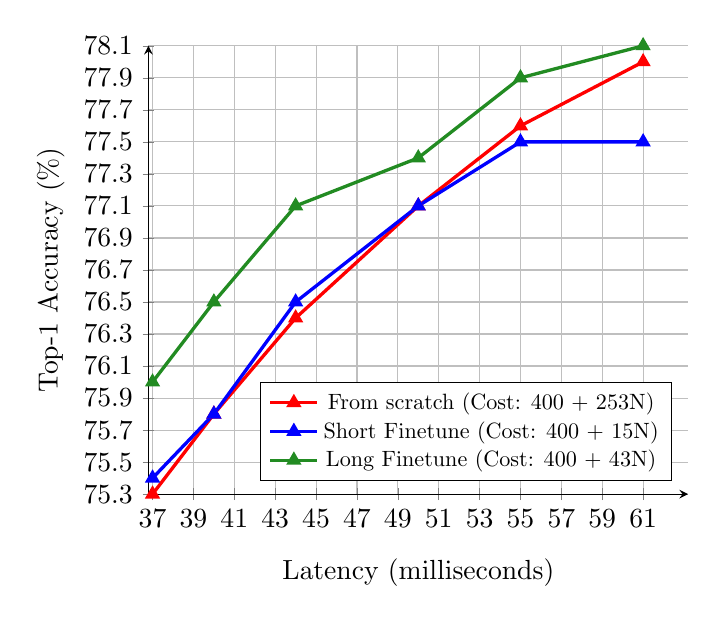
\begin{tikzpicture}
\begin{axis}[
axis x line=left,
            axis y line=left,
            xmajorgrids=true,
            ymajorgrids=true,
            grid=both,
            xlabel style={below=1ex},
            enlarge x limits,
            ymin = 75.3,
            ymax = 78.1,
xmin = 39.0,
            xmax = 61.0,
xtick = {37,39,...,61},
ytick = {75.3,75.5,...,78.1},
            ylabel = Top-1 Accuracy (\%),
            xlabel = Latency  (milliseconds),
            legend pos=south east,
            legend style={nodes={scale=0.8, transform shape}},
            legend pos=south east,
    ]




\addplot[color=red, mark=triangle*,very thick]coordinates {(37, 75.3)(40,75.8)(44, 76.4)(50, 77.1)(55, 77.6)(61,78.0)};\addlegendentry{From scratch (Cost: 400 + 253N)}



\addplot[color=blue, mark=triangle*,very thick]coordinates {(37, 75.4)(40,75.8)(44, 76.5)(50, 77.1)(55, 77.5)(61,77.5)};\addlegendentry{Short Finetune (Cost: 400 + 15N)}

\addplot[color=ForestGreen, mark=triangle*,very thick]coordinates {(37, 76.0)(40,76.5)(44, 77.1)(50, 77.4)(55, 77.9)(61,78.1)};\addlegendentry{Long Finetune (Cost: 400 + 43N)}



























\end{axis}
\end{tikzpicture}
\end{adjustbox}
\vspace{-5mm}
\caption{Top-1 accuracy on Imagenet vs Latency measured on Intel Xeon CPU for a batch size of 1, for architectures found with our method trained from scratch and fine-tuned from the pretrained super-network}
\label{fig:acc_nas2}
\end{figure}
\vspace{-3mm}
%
 
\section{Solving the Mathematical Programs Requires a Negligible Computation Time}
In this section we measure the computation time for solving the mathematical programs associated with the initialization point, the LP associated with the FW step and the LP associated with our projection.
We show that the measured times are negligible compared to the computation time attributed to backpropagation.

The average time, measured during the search, for solving the linear programs specified in Algorithm~\ref{alg:BCSFW} and in Section~\ref{sec:projection} and the quadratic program specified in Appendix~\ref{sec:init_point} is  CPU hours.

The average time, measured during the search, for a single backpropagation of gradients through the one-shot model is  GPU Hours.

The overall cost of solving the mathematical programs for generating  networks is about  CPU hours, which is negligible compared to the overall  GPU hours.
 \end{document}